\documentclass[11pt]{article}

\usepackage{centernot}
\usepackage{amssymb}
\usepackage{xcolor}
\definecolor{myblue}{RGB}{0, 0, 255} 
\definecolor{mygreen}{RGB}{0, 180, 80}
\definecolor{myred}{RGB}{153, 0, 0}
\definecolor{myorange}{RGB}{255, 153, 51}
\definecolor{mypurple}{RGB}{102, 0, 204}
\usepackage{verbatim}
\usepackage{multicol}
\usepackage{enumitem}
\usepackage{amsfonts}
\usepackage{amsmath}
\usepackage[utf8]{inputenc}
\usepackage[export]{adjustbox}  % for correct logo rendering
\usepackage{fancyhdr}  % for header/footer formatting
\usepackage{hyperref}  % for hyper-references
\usepackage{datetime}  % to update month in footer
\usepackage{array}  % more flexible tables
\usepackage[includeheadfoot,
            left=1in,
            right=1in,
            top=0.75in,
            bottom=0.75in,
            headheight=40pt]{geometry} % geometry needs to know headheight to correctly render the footer
\usepackage{tikz} % For drawing grid boxes

\definecolor{darkblue}{RGB}{0, 0, 139}
\definecolor{lightblue}{RGB}{173, 216, 230}

% desired format for footer
\newdateformat{monthyeardate}{%
  \monthname[\THEMONTH] \THEYEAR}

% set up header/footer
\pagestyle{fancy}
\fancyhf{}  % clear all headers/footers
\renewcommand{\headrulewidth}{0pt}  % remove header rule
\renewcommand{\footrulewidth}{0pt}  % remove footer rule

% set up header

\fancypagestyle{firstpage}{
    \fancyhead[L]{
    \vspace{0pt}
    \hspace{-8pt}
    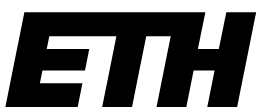
\includegraphics[width=0.1\textwidth]{docimgs/eth_logo_kurz_pos.png}\\
    \textbf{Swiss Federal Institute of Technology}\\
    \textbf{Zurich}\\
    %\textbf{ } \\
    
    }    

    \fancyhead[R]{
    \raggedleft
    %\vspace{20pt}
    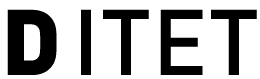
\includegraphics[width=0.13\textwidth]{docimgs/eth_ditet_logo_pos.png}\\
     \textbf{Dept. of Information Technology and} \\ \textbf{Electrical Engineering}  \\
     %\textbf{Chair for Mathematical Information} \\ \textbf{Information Science} \\

    }
}

% set up footer
\fancyfoot[L]{mdietz, ÜS 9}
\fancyfoot[C]{\thepage}
\fancyfoot[R]{\monthyeardate\today}

% set up section/subsection titles
\renewcommand{\thesection}{\arabic{section}}
\renewcommand{\thesubsection}{\arabic{subsection}}

% command used for simply emphasizing suggestions
\newcommand{\suggestion}[1]{{\itshape #1}}

%--- commands for transform arrows----------------
\newcommand{\transform}[2]{%
    \begin{tikzpicture}
        % Open circle
        \draw[thick] (0,0) circle (0.1);
        % Line with number above and adjustable length
        \draw[thick] (0.1,0) -- (#2,0) node[midway, above] {#1};
        % Filled circle
        \filldraw[thick] (#2,0) circle (0.1);
    \end{tikzpicture}%
}
\newcommand{\invtransform}[2]{%
    \begin{tikzpicture}
        % filled circle
        \filldraw[thick] (0,0) circle (0.1);
        % Line with number above and adjustable length
        \draw[thick] (0.1,0) -- (#2 -0.1,0) node[midway, above] {#1};
        % open circle
        \draw[thick] (#2,0) circle (0.1);
    \end{tikzpicture}%
}
\newcommand{\verticaltransform}[4]{%
    \begin{tikzpicture}
        % Open circle at the bottom with text below
        \filldraw[thick] (0,0) circle (0.1) node[below=3pt] {$#4$};
        % Vertical line with number on the left
        \draw[thick] (0,0.1) -- (0,#2 -0.1) node[midway, left] {#1};
        % Filled circle at the top with text above
        \draw[thick] (0,#2) circle (0.1) node[above=3pt] {$#3$};
    \end{tikzpicture}%
}
\newcommand{\verticalinvtransform}[4]{%
    \begin{tikzpicture}
        % Open circle at the bottom with text below
        \draw[thick] (0,0) circle (0.1) node[below=3pt] {$#4$};
        % Vertical line with number on the left
        \draw[thick] (0,0.1) -- (0,#2) node[midway, left] {#1};
        % Filled circle at the top with text above
        \filldraw[thick] (0,#2) circle (0.1) node[above=3pt] {$#3$};
    \end{tikzpicture}%
}

\begin{document}
\thispagestyle{firstpage}

\setlength{\headheight}{1 \baselineskip}  % accomodate header
\setlength{\parindent}{0pt}  % remove initial paragraph indent
\setlength{\parskip}{\baselineskip}  % add skip between paragraphs

\vspace*{-5px}
\section*{Übungsstunde 9}

\section*{Themenüberblick}
\begin{itemize}
    \item \textbf{Repetition: Abtasttheorem}
    \item \textbf{Zeitdiskrete Signale und Systeme}
    \item[] Zeitdiskrete Fouriertransformation (DTFT)
    \item[] Zeitdiskrete LTI-Systeme und Systemeigenschaften
    \item[] Differenzengleichungen
\end{itemize}

\section*{Aufgaben für diese Woche}
\vspace{-0.5cm}

\textbf{97}, 98, 99, 100, 101, \textbf{102}, \textbf{103}, \textbf{104}, 105, 106, \textbf{107}, \textbf{108}, 109, \textbf{110}, \textbf{111}, \textbf{112}, 113\\
\vspace{-0.5cm}

Die \textbf{fettgedruckten} Übungen empfehle ich, weil sie wesentlich zu eurem Verständnis der Theorie beitragen und/oder sehr prüfungsrelevant sind.

\vfill \null
\pagebreak

\section*{Repetition: Abtasttheorem}
\vspace*{-0.5cm}
\subsection*{Abgetastete Signale im Frequenzbereich}
\vspace*{-0.5cm}
$$x_{abg.}(t) = x(t)\delta_T(t) = \sum_{k=-\infty}^{\infty} x(kT)\delta(t-kT) \hspace{10pt} \transform{20.}{2} \hspace{10pt} \hat{x}_{abg.}(f) = \frac{1}{T} \sum_{k = -\infty}^\infty \hat{x}\left( f- \frac{k}{T} \right)$$
\vspace*{-0.5cm}
\begin{center}
    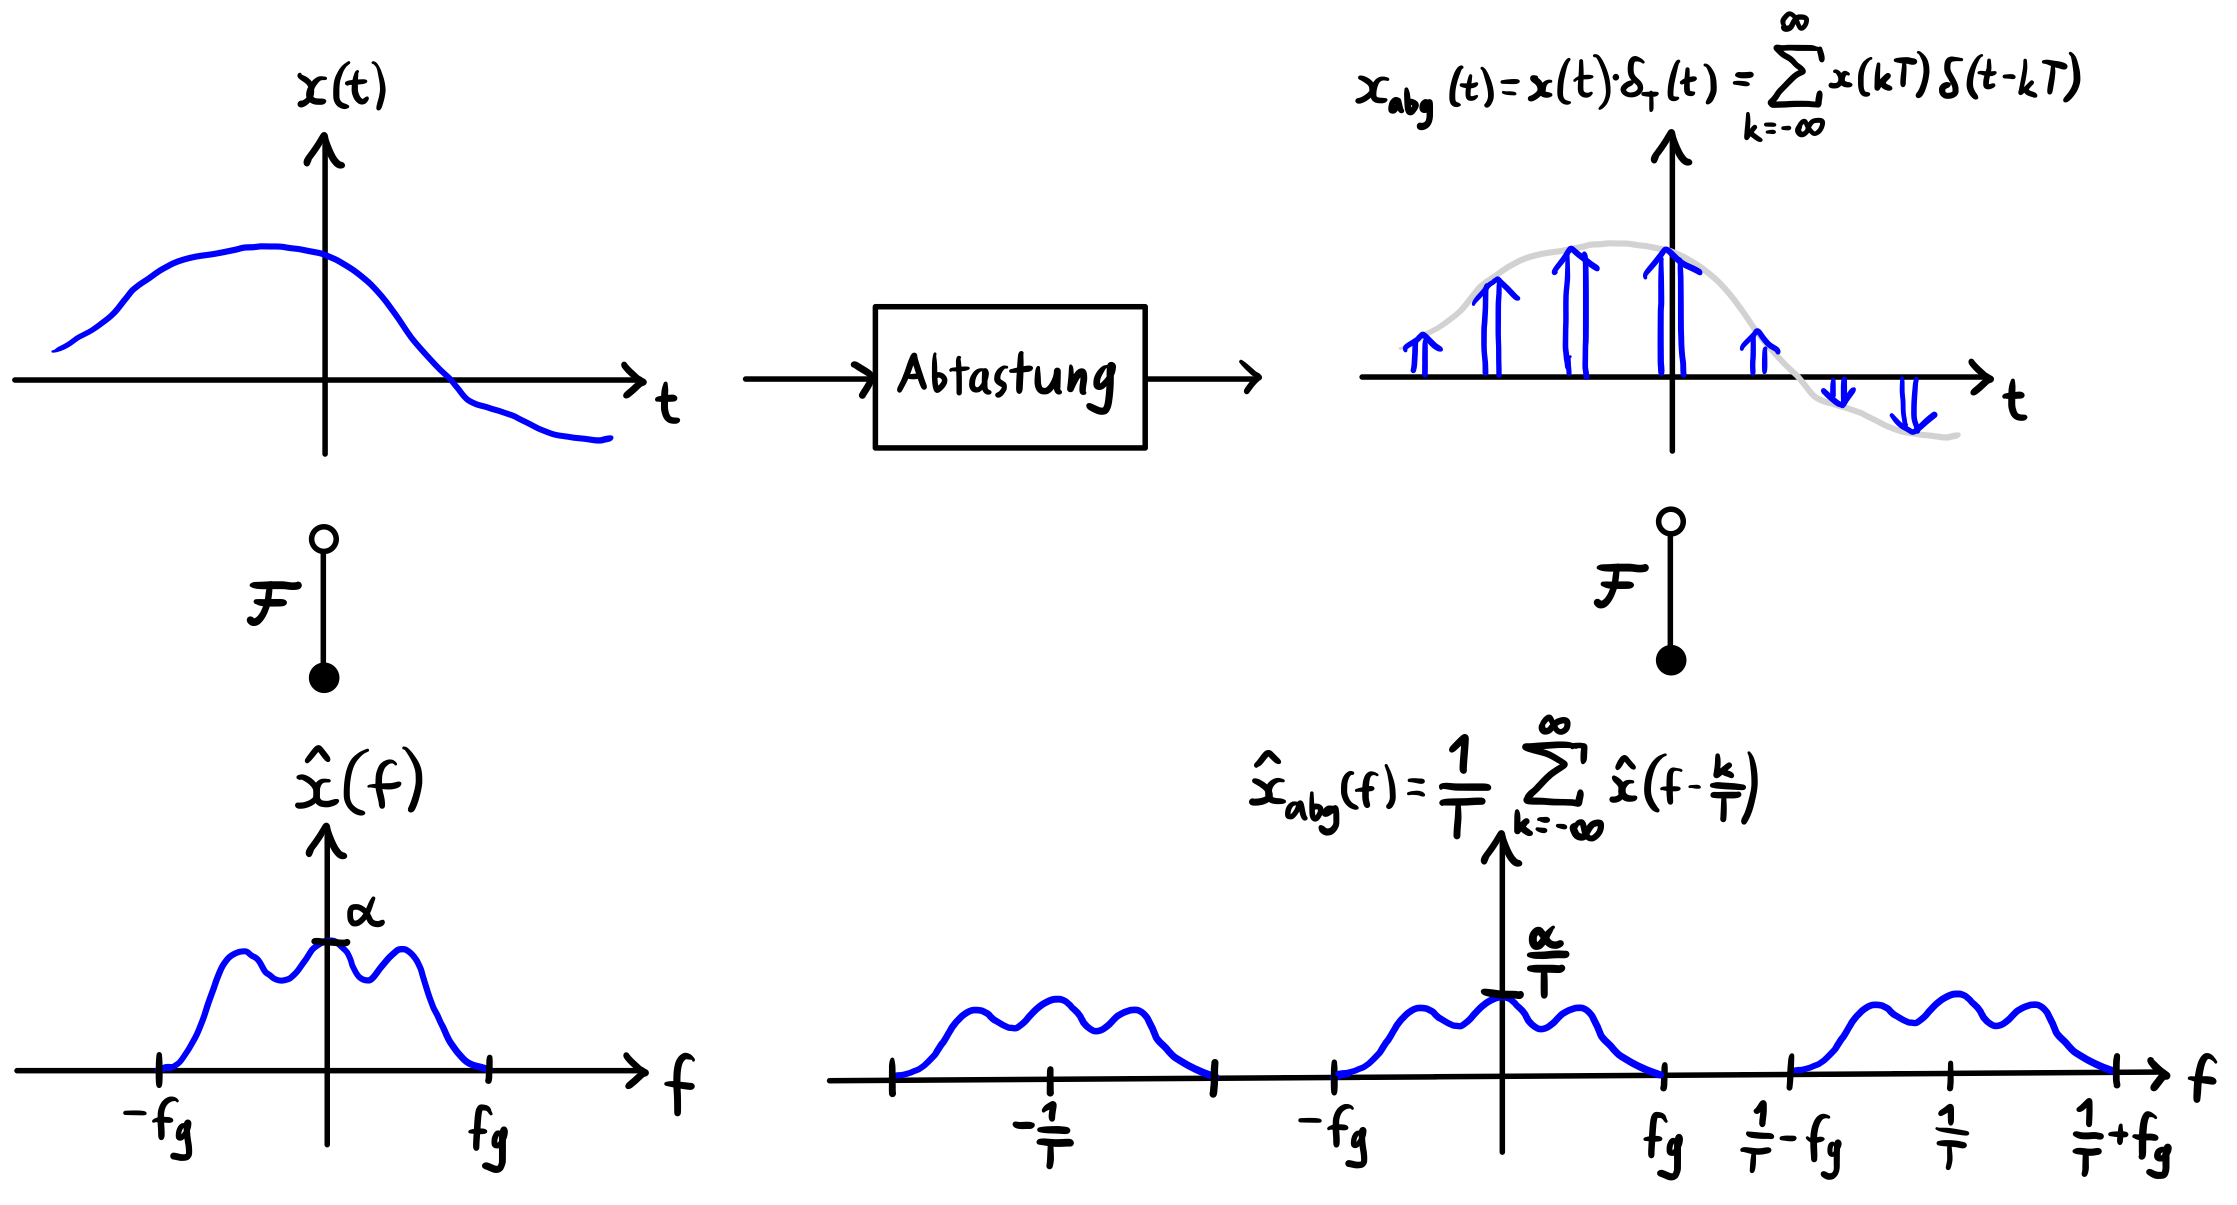
\includegraphics[width=0.8\linewidth]{docimgs/abtastung2.jpg}
\end{center}
\vspace*{-0.75cm}
\begin{itemize}[leftmargin=0pt]
    \item[] \fcolorbox{darkblue}{lightblue}{%
    \parbox{\dimexpr\linewidth-2\fboxsep-2\fboxrule\relax}{
        Die Abtastung im Zeitbereich entspricht einer Periodisierung im Frequenzbereich.
    }}%
    \item[]  Die Abtastung von $x(t)$ erzeugt im Frequenzbereich um Skalierungsfaktor $\frac{1}{T}$ skalierte Kopien von $\hat{x}(f)$, die um $f_s = \frac{1}{T}$ verschoben sind, wobei $T$ die Abtastperiode ist.
\end{itemize}

\noindent
\begin{minipage}[t]{0.32\textwidth}
    \begin{center}
        \textbf{Kritische Abtastung}
    \end{center}
    \vspace*{-0.5cm}
    \begin{center}
        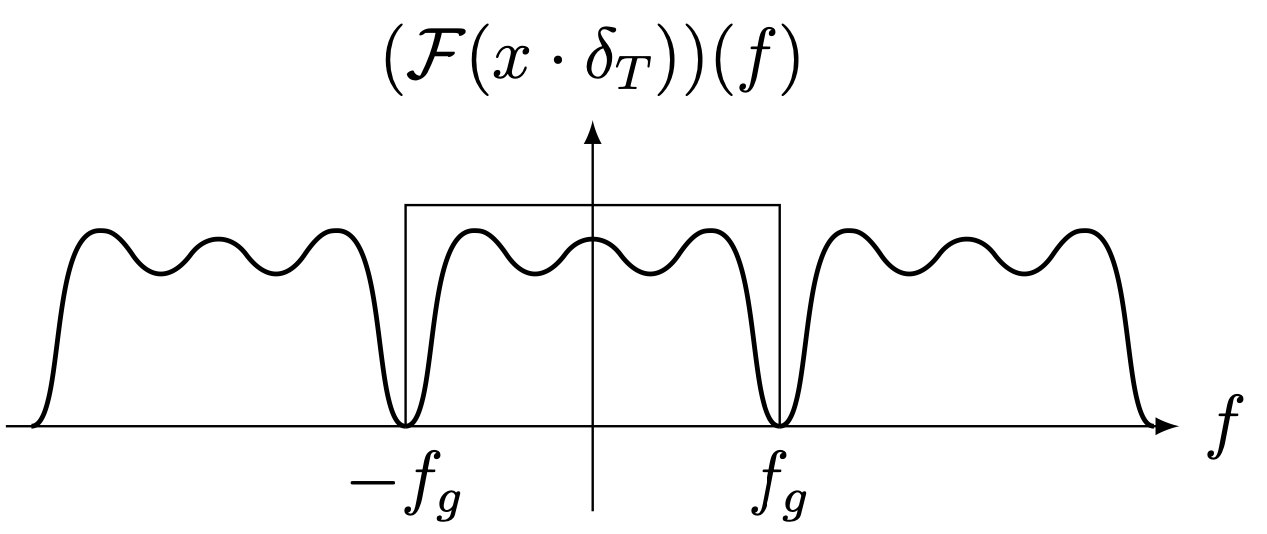
\includegraphics[width=0.77\linewidth]{docimgs/krit_abtast.png}
    \end{center}
    $$f_s = 2f_g$$
    Wir können das Signal mit einem idealen Tiefpassfilter der Breite $W = f_g$ rekonstruieren.
\end{minipage}
\hfill
\begin{minipage}[t]{0.32\textwidth}
    \begin{center}
        \textbf{Überabtastung}
    \end{center}
    \vspace*{-0.5cm}
    \begin{center}
        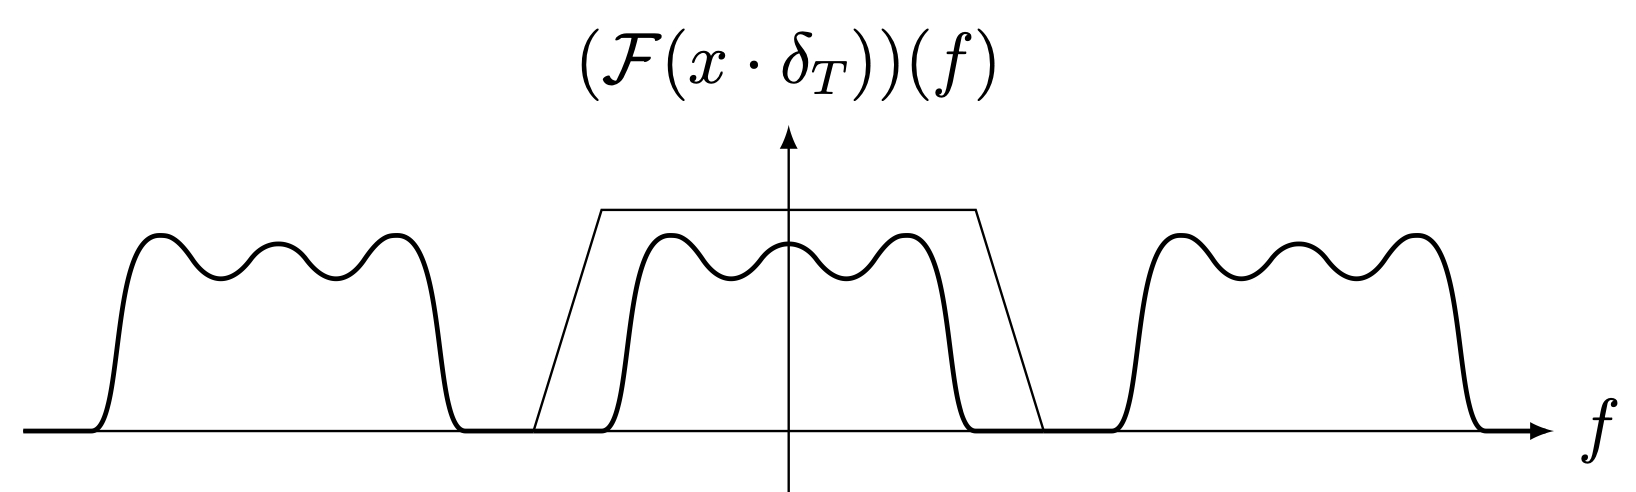
\includegraphics[width=\linewidth]{docimgs/ueberabtast.png}
    \end{center}
    $$f_s > 2f_g$$
    In diesem Fall können wir sogar einen stabilen Tiefpassfilter verwenden. Überabtastung mit $f_s > 2f_g$ garantiert nicht nur, dass perfekte Rekonstruktion möglich ist, sondern hilft im Allgemeinen auch, die Empfindlichkeit auf Rauschen im Abtastprozess zu verringern.
\end{minipage}
\hfill
\begin{minipage}[t]{0.32\textwidth}
    \begin{center}
        \textbf{Unterabtastung}
    \end{center}
    \vspace*{-0.5cm}
    \begin{center}
        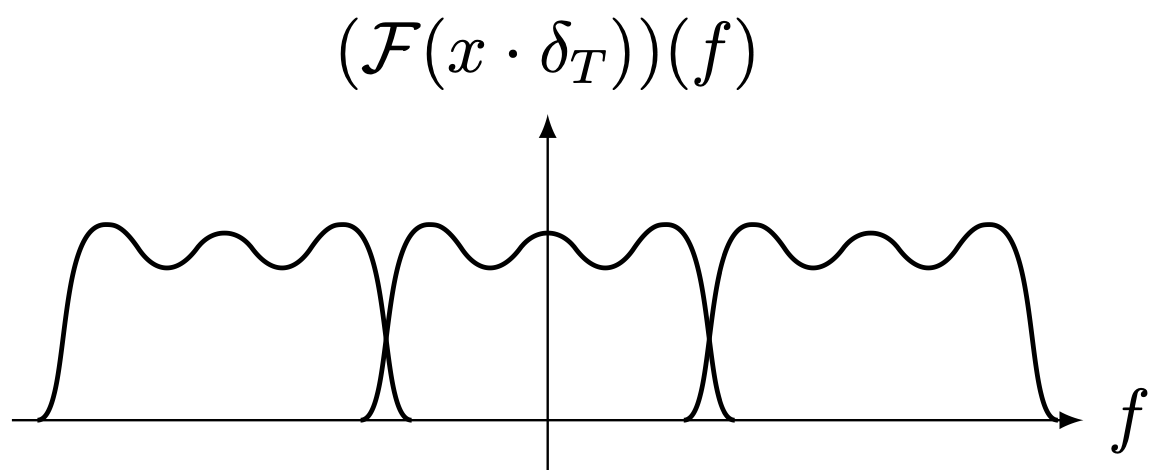
\includegraphics[width=0.75\linewidth]{docimgs/aliasing1.png}
    \end{center}
    $$f_s < 2f_g$$
    Es gibt \textbf{Aliasing}. Mit Hilfe eines Tiefpassfilters erhalten wir keine perfekte Version von $\hat{x}(f)$, eine Rekonstruktion des ursprünglichen Signals ohne Informationsverluste ist somit nicht möglich.
\end{minipage}

\pagebreak

\subsection*{Abtasttheorem}
\vspace*{-0.5cm}
\fcolorbox{darkblue}{lightblue}{%
    \parbox{\dimexpr\linewidth-2\fboxsep-2\fboxrule\relax}{
        \vspace*{0.25cm}
        Ein Signal mit der Bandbreite $f_g$ kann aus seinen Abtastwerten, genommen mit einer Rate von $f_s \geq 2f_g$, eindeutig rekonstruiert werden. Die kritische Rate $f_s = 2 f_g$ wird als \textbf{Nyquistrate} bezeichnet.
        \vspace*{0.25cm}
    }}%

\subsection*{Rekonstruktion}
\begin{itemize}[leftmargin=0pt]
    \item[] Im Allgemeinen ist die Rekonstruktion eines Signals aus seinen Abtastwerten gegeben durch:
    \item[] 
    \fcolorbox{darkblue}{lightblue}{%
    \parbox{\dimexpr\linewidth-2\fboxsep-2\fboxrule\relax}{
       $$y(t) = T \displaystyle\sum_{k = -\infty}^\infty x(kT)h(t-kT)$$
    }}%
    \item[] wobei $h(t)$ die Impulsantwort eines Filters ist. Im Falle der kritischen Abtastung brauchen wir für die Rekonstruktion einen idealen Tiefpassfilter $h(t) = h_{id}(t)$ mit Breite $W = f_g = \frac{f_s}{2} = \frac{1}{2T}$.
    $$\hat{h}_{id}(f) = \displaystyle\begin{cases}
        1, \; |f| \leq W \\
        0, \; |f| > W
    \end{cases} \invtransform{}{1} \; h_{id}(t)=\displaystyle\frac{\sin(2 \pi W t)}{\pi t}$$
    \item[] Deswegen gilt bei der kritischen Abtastung: $y(t) = x(t) = \displaystyle\sum_{k=-\infty}^\infty x(kT)\displaystyle\frac{\sin\left(\frac{\pi}{T}(t-kT)\right)}{\frac{\pi}{T}(t-kT)}$
\end{itemize}
\vspace*{-0.75cm}
\begin{center}
    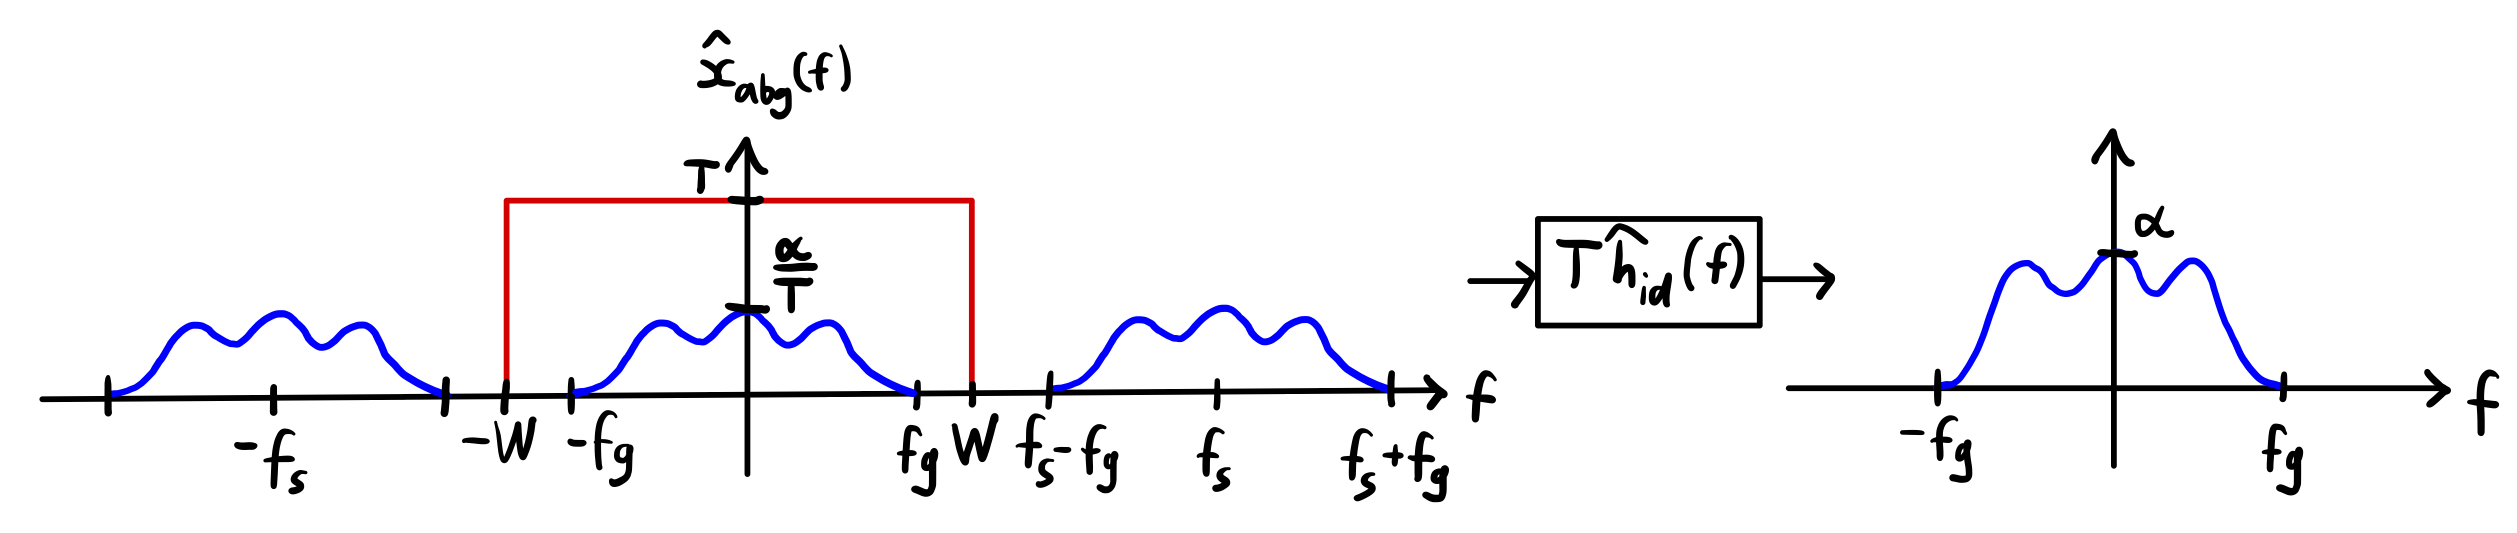
\includegraphics[width=\linewidth]{docimgs/filtering1.jpg}
\end{center}

\vfill \null
\pagebreak

\section*{Zeitdiskrete Signale}
\vspace*{-0.5cm}
Eine Abtastung im Zeitbereich ergibt eine periodische Fortsetzung des Spektrums, d.h.
$$\hat{x}_{\text{abg}}(f) = \mathcal{F}\{x \cdot \delta_T\}(f) = \frac{1}{T}\sum_{k=-\infty}^{\infty}\hat{x}\left( f- \frac{k}{T} \right)$$
Dieses Signal ist $\frac{1}{T}-$periodisch und besitzt somit eine Fourierreihendarstellung. Wir verwenden im Folgenden die Poissonsche Summenformel und die Dualität der Fouriertransformation.

\noindent
\begin{minipage}[t]{0.48\textwidth} % Left column
    \textbf{Poissonsche Summenformel}\\[0.5em]
    \[
    \sum_{k=-\infty}^\infty h(t + kT) = \frac{1}{T} \sum_{k=-\infty}^\infty \hat{h}(k/T)e^{2 \pi i k t/T}
    \]
    \[
    \text{Substitution: }h \to \hat{x}, \; t \to f, \; T \to \frac{1}{T}
    \]
\end{minipage}
\hfill
\begin{minipage}[t]{0.48\textwidth} % Right column
    \textbf{Dualität der Fouriertransformation}\\[0.5em]
    \includegraphics[width=0.6\textwidth]{docimgs/dualität_1.png}
\end{minipage}

$$\implies \frac{1}{T}\sum_{k=-\infty}^{\infty}\hat{x}\left( f- \frac{k}{T} \right) = \frac{1}{T}\cdot T \sum_{k=-\infty}^{\infty} \underbrace{\hat{\hat{x}}(kT)}_{x(-kt)}e^{2 \pi i k f T} = \sum_{k=-\infty}^\infty x(-kT)e^{2 \pi i k f T} = \sum_{k=-\infty}^\infty \underbrace{x(kT)}_{c_k}e^{-2 \pi i k f T}$$
Indem wir im letzen Schritt die Summationsreihenfolge gewechselt haben $(k \to -k)$, haben wir das abgetastete Signal im Frequenzbereich $\hat{x}_{\text{abg}}(f)$ als komplexe Fourierreihe dargestellt. Die \textbf{Abtastwerte} $x(kT)$ sind die Koeffizienten der Fourierreihe des Spektrums $\hat{x}_{\text{abg}}(f)$.

\subsection*{Notation für Zeitdiskrete Signale}
\vspace*{-0.5cm}
\fcolorbox{black}{white}{\color{black} $x_d[k] := x(kT)$, wobei $k \in \mathbb{Z}$, nimmt nur ganze Zahlen als Argument}

\begin{center}
    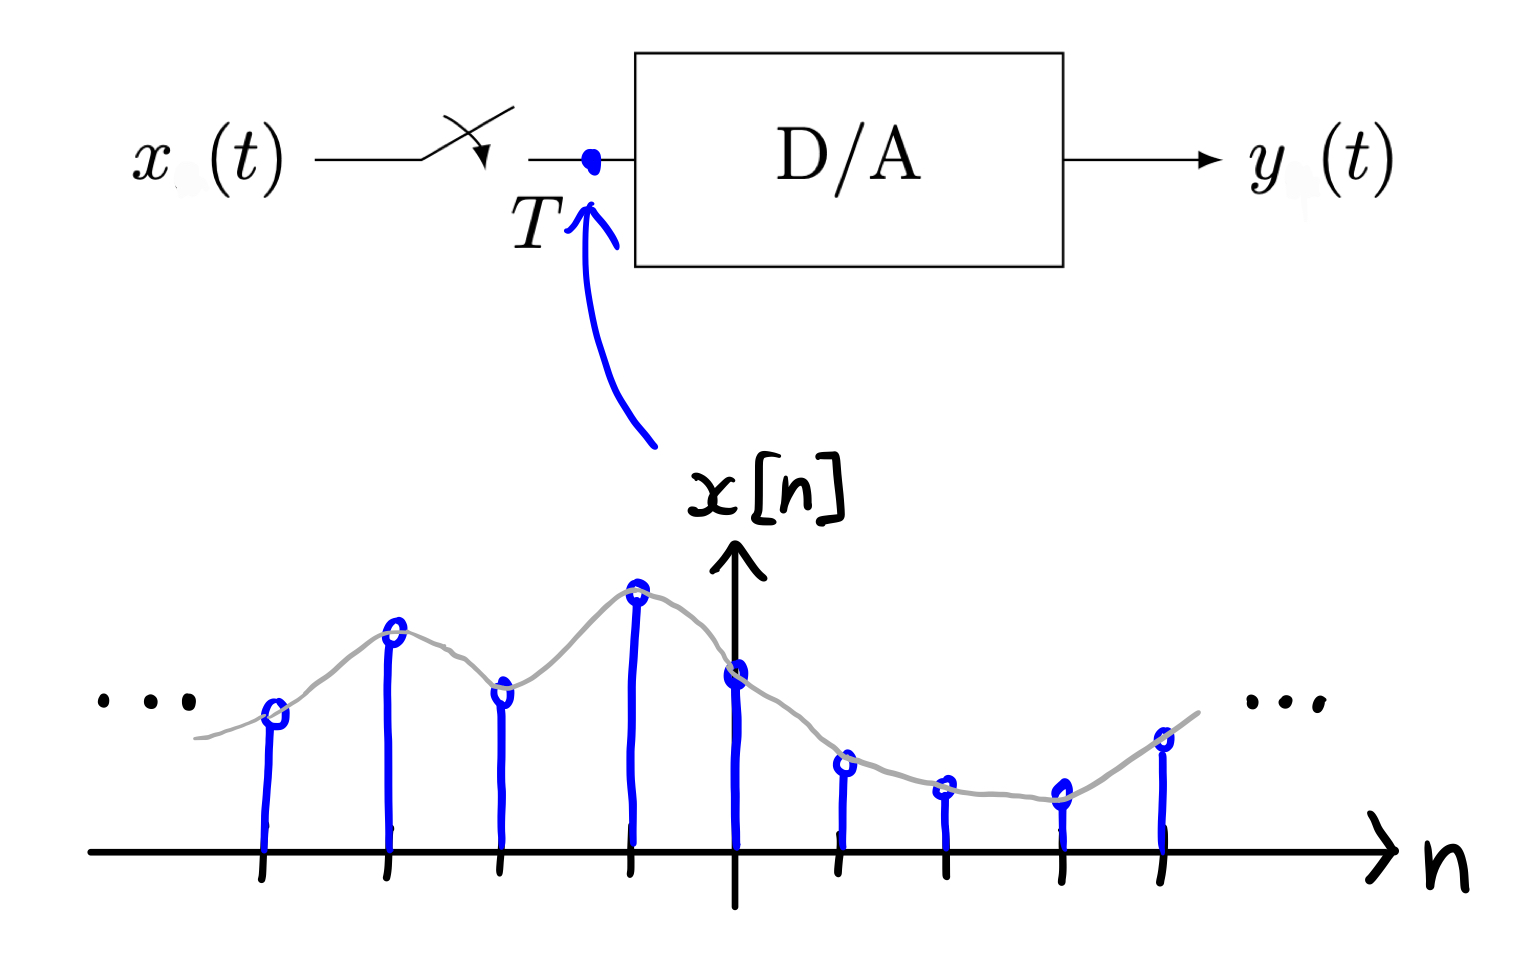
\includegraphics[width=0.6\linewidth]{docimgs/abtast.jpg}
\end{center}

\pagebreak

\subsection*{Zeitdiskrete Signale im Frequenzbereich}
\vspace*{-0.5cm}
Wir definieren $\theta = Tf$ und erhalten somit mithilfe der Formel von oben
$$\sum_{k=-\infty}^\infty x_d[k] e^{-2\pi i k \theta} = \sum_{k=-\infty}^\infty x(kT) e^{-2\pi i k T f} = \frac{1}{T}\sum_{k=-\infty}^{\infty}\hat{x}\left( f- \frac{k}{T} \right) = \frac{1}{T}\sum_{k=-\infty}^{\infty}\hat{x}\left( \frac{\theta - k}{T} \right) = \hat{x}_d(\theta)$$

\begin{itemize}[leftmargin = 0pt]
    \item[] Somit erhalten wir die Zeitdiskrete Fouriertransformation (\textit{Discrete Time Fourier Transform}):
    \item[] \fcolorbox{darkblue}{lightblue}{%
    \parbox{\dimexpr\linewidth-2\fboxsep-2\fboxrule\relax}{\begin{itemize}
        \item[] $(\textbf{DTFT}) \hspace{80pt} \hat{x}_d(\theta) = \displaystyle\sum_{n=-\infty}^\infty x_d[n]e^{-2 \pi i n \theta}$
        \item[] $(\textbf{IDTFT}) \hspace{76pt} x_d[n]=\displaystyle\int_0^1 \hat{x}_d(\theta)e^{2 \pi i n \theta} \text{d}\theta$
    \end{itemize}
}}%
   \item[] \textbf{Rücktransformation}:
   \begin{align*}
       \int_0^1 \hat{x}_d(\theta) \cdot e^{2 \pi i n \theta}\text{d}\theta &= \int_0^1 \left( \sum_{l=-\infty}^\infty x_d[l]e^{-2\pi i l \theta} \right)\cdot e^{2 \pi i n \theta} \text{d}\theta = \underbrace{\sum_{l=-\infty}^\infty x_d[l]}_{\text{unabhg. von }\theta} \cdot \underbrace{\int_0^1 e^{2 \pi i (n-l)\theta} \text{d}\theta}_{\delta[n-l]} \\
       &= \sum_{l=-\infty}^\infty x_d[l]\delta[n-l] = x_d[n]
   \end{align*}
    \item[] \textbf{Bemerkungen}:
\end{itemize}
\vspace*{-1cm}
\begin{itemize}
    \item Die DTFT transformiert ein Signal von einem \textbf{diskreten Zeitbereich} in einen \textbf{kontinuierlichen Frequenzbereich}.
    \item $\theta = Tf = \frac{f}{f_s}$ ist die \textbf{relative Frequenz}. ($T=$ Abtastperiode und $f_s=$ Abtastfrequenz)
    \item $\hat{x}_d(\theta) = \displaystyle\frac{1}{T} \sum_{k=-\infty}^\infty \hat{x}\left( \frac{\theta - k}{T} \right)$ ist \textbf{1-periodisch} in $\theta$.
    \item[]  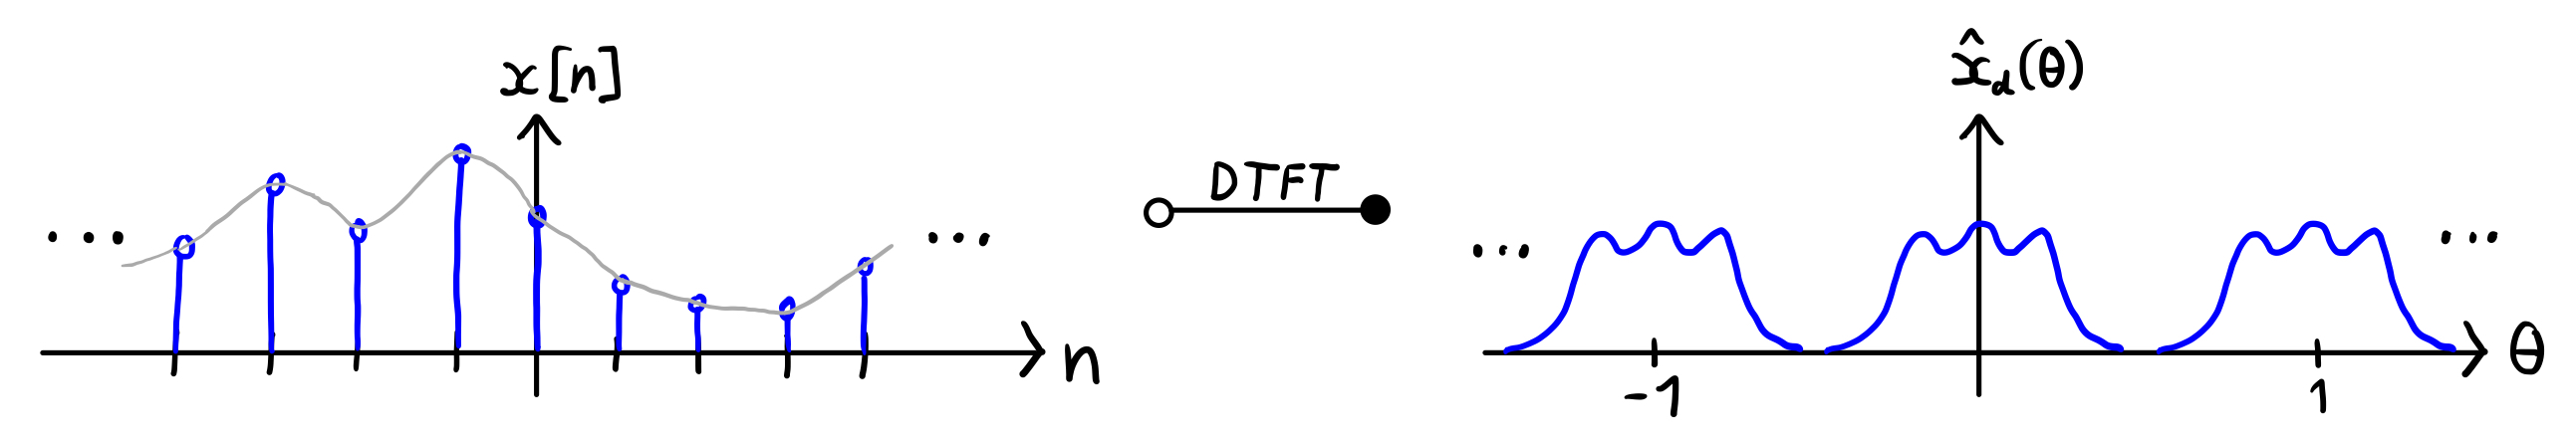
\includegraphics[width=\linewidth]{docimgs/dtft.jpg}
\end{itemize}

\vfill \null
\pagebreak

\section*{Formelsammlung: Fouriertransformation zeitdiskreter Signale (DTFT)}
\vspace*{-0.75cm}
\begin{center}
    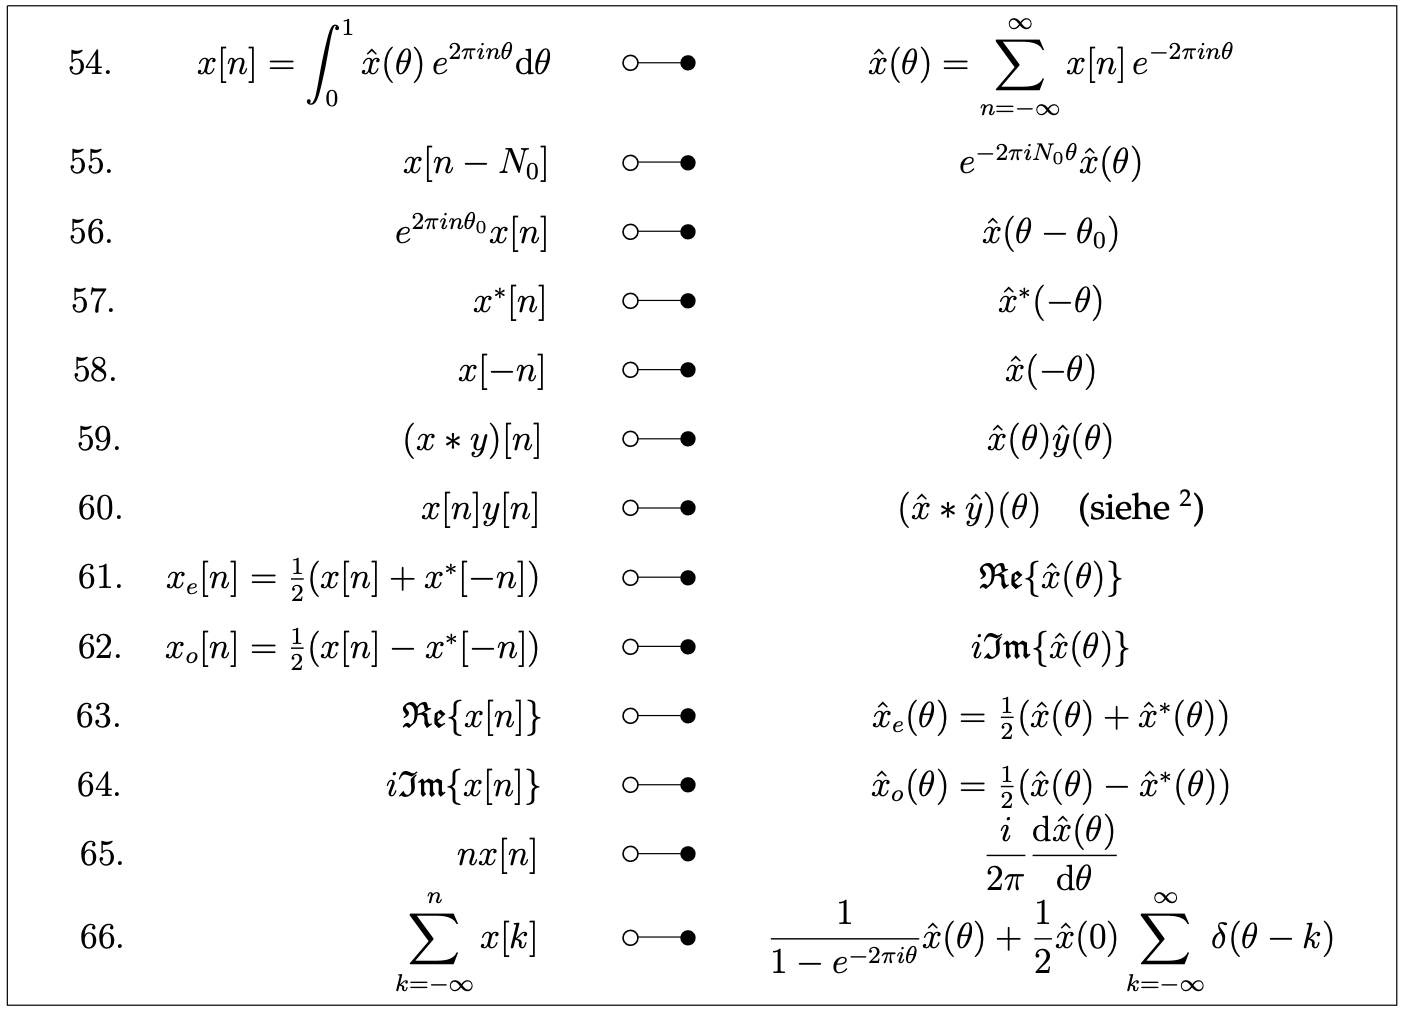
\includegraphics[width=0.87\linewidth]{docimgs/DTFT.png}\\
    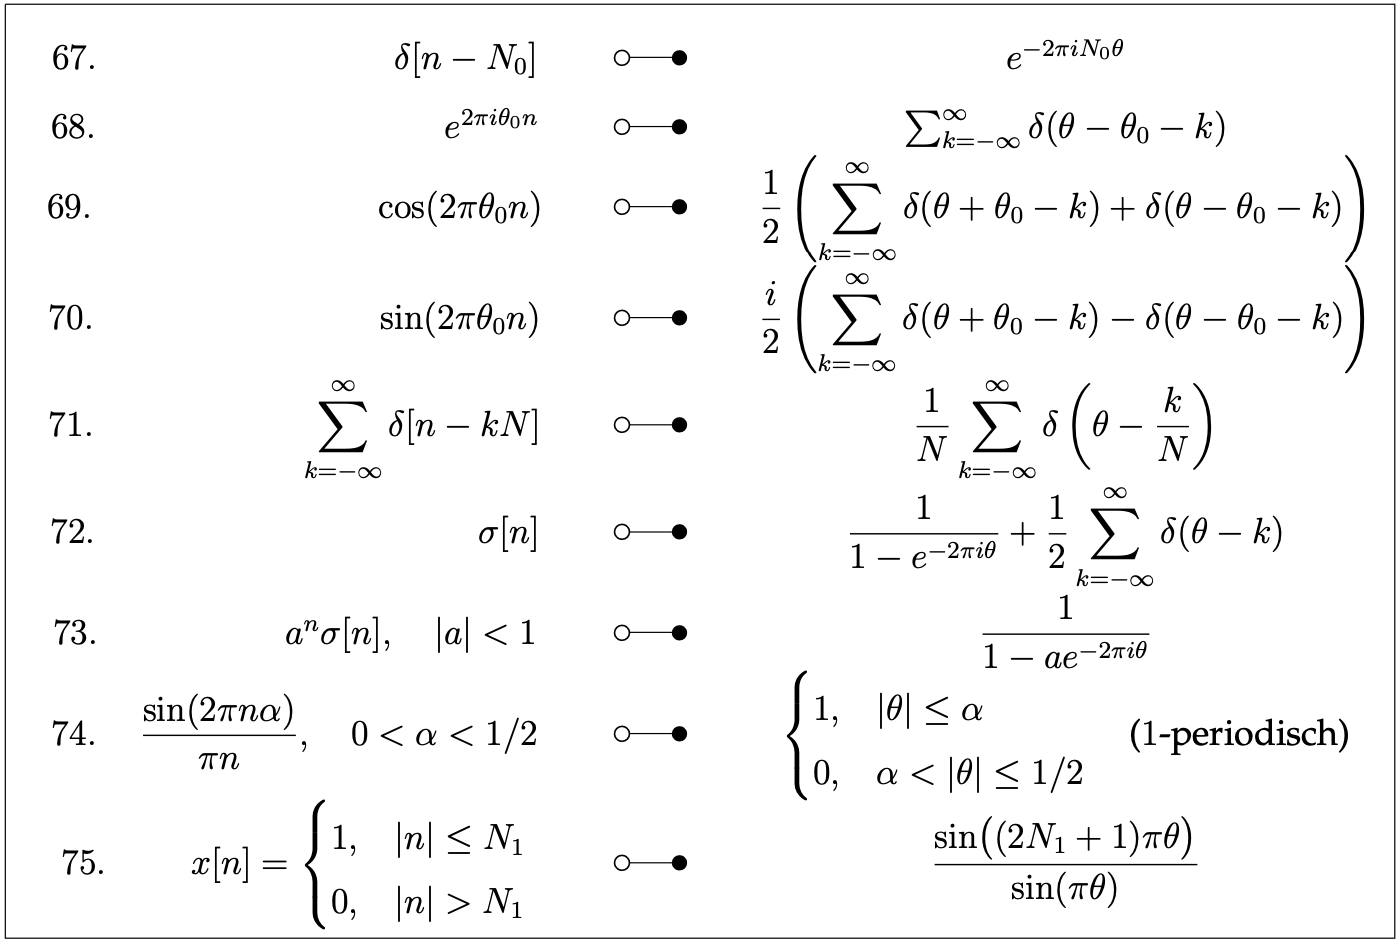
\includegraphics[width=0.867\linewidth]{docimgs/DTFT_paare.png}
\end{center}

\pagebreak

\section*{Zeitdiskrete Systeme}
\vspace*{-0.5cm}
\begin{center}
    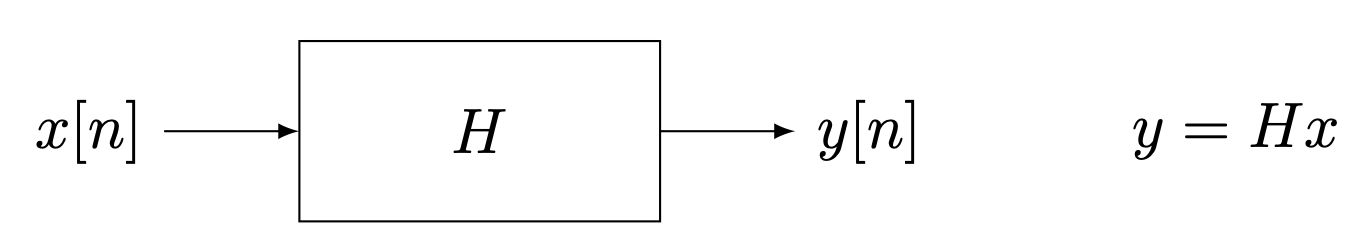
\includegraphics[width=0.55\linewidth]{docimgs/System_zeitdiskret.png}
\end{center}
\vspace*{-0.5cm}
Die folgenden Eigenschaften sind im zeitdiskreten Bereich analog definiert wie im zeitkontinuierlichen. (Vgl. ÜS 3)
\vspace*{-0.75cm}
\subsection*{Linearität}
\vspace*{-0.5cm}
\begin{itemize}
    \item $H(\alpha x_1 + x_2) = \alpha H x_1 + H x_2 \hspace{16pt} \forall x_1, x_2 \in X, \; \forall \alpha \in \mathbb{C}$
\end{itemize}
\vspace*{-0.75cm}
\subsection*{Zeitinvarianz}
\vspace*{-0.5cm}
\begin{itemize}
    \item $H(x[\cdot -n_0]) = (Hx)[\cdot -n_0] \hspace{16pt} \forall x\in X, \; \forall n_0 \in \mathbb{Z}$
\end{itemize}
\vspace*{-0.75cm}
\subsection*{Kausalität}
\vspace*{-0.5cm}
\begin{itemize}
    \item $x_1[n] = x_2[n] \hspace{10pt} \forall n \leq n_0 \implies (Hx_1)[n] = (Hx_2)[n] \hspace{10pt} \forall n \leq n_0 \hspace{16pt} \forall x_1, x_2 \in X, \; \forall n_0 \in \mathbb{Z}$
\end{itemize}
\vspace*{-0.75cm}
\subsection*{BIBO-Stabilität}
\vspace*{-0.5cm}
\begin{itemize}
    \item $\forall x \in X$ mit $|x[n]| \leq B_x < \infty \hspace{10pt} \forall n \in \mathbb{Z} \implies \exists B_y < \infty$ mit $ |(Hx)[n]| \leq B_y \hspace{10pt} \forall n \in \mathbb{Z}$
\end{itemize}

\subsection*{Kronecker-Delta Funktion}
\vspace*{-0.5cm}
Die Kronecker-Delta Funktion ist definiert als
$$\delta[n] = \begin{cases}
    1, \hspace{12pt} n = 0 \\
    0, \hspace{12pt} n \neq 0
\end{cases} \hspace{20pt} \text{bzw.} \hspace{20pt} \delta[n-n_0] = \begin{cases}
    1, \hspace{12pt} n = n_0 \\
    0, \hspace{12pt} n \neq n_0
\end{cases}$$
Es gilt $x[n] = \displaystyle\sum_{k=-\infty}^\infty x[k]\delta[n-k]$

\subsection*{Zeitdiskrete LTI-Systeme}
\vspace*{-0.5cm}
Ein zeitdiskretes System ist LTI, wenn es linear und zeitinvariant ist. Die Systemantwort von zeitdiskreten LTI-Systemen lautet:
$$y[n] = (Hx)[n] = H\left( \sum_{k=-\infty}^\infty x[k] \delta[\cdot - k] \right)[n] \overset{\text{Lin.}}{=} \sum_{k=-\infty}^\infty x[k]\left( H (\delta[\cdot - k]) \right)[n] \overset{\text{Zeitinv.}}{=} \sum_{k = -\infty}^\infty x[k]\underbrace{(H\delta)[n-k]}_{=:h[n-k]}$$
Die zeitdiskrete Impulsantwort ist definiert als $h[n] = (H\delta)[n]$

\pagebreak

\begin{itemize}[leftmargin=0pt]
    \item[] Die Antwort von einem LTI-System ist also:
    \item[] \fcolorbox{darkblue}{lightblue}{%
    \parbox{\dimexpr\linewidth-2\fboxsep-2\fboxrule\relax}{
    $$\hspace{10pt}y[n] = \displaystyle\sum_{k=-\infty}^\infty x[k]h[n-k] = \displaystyle\sum_{k=-\infty}^\infty x[n-k]h[k] \hspace{8pt}\underset{59}{\transform{DTFT}{1.5}}\hspace{8pt} \hat{y}(\theta) = \hat{x}(\theta)\hat{h}(\theta)$$
}}%
\end{itemize}

\vspace*{-0.5cm}
\subsection*{Systemeigenschaften Zeitdiskreter LTI-Systeme}
\vspace*{-0.5cm}
Ein LTI-System heisst ...
\vspace*{-0.25cm}
\begin{itemize}
    \item \textbf{kausal}, genau dann wenn:  $h[n] = 0 \hspace{10pt} \forall n < 0$
    \item \textbf{BIBO-stabil}, wenn: $\displaystyle\sum_{n=-\infty}^\infty |h[n]| < \infty$, (also $h \in l^1$)
\end{itemize}

\vspace*{-0.5cm}
\subsection*{Prüfungsaufgabe Frühjahr: 2017, Aufgabe 3.a)}
\begin{itemize}
    \item[a)] (14 Punkte) Wir betrachten das zeitdiskrete LTI-System $H_1$ mit der Impulsantwort
    $$h_1[n] = 4 \left( \left( \frac{1}{2}\right)^n - \left(-\frac{1}{3} \right)^n \right)\sigma[n]$$
    \begin{itemize}
        \item[i.] Bestimmen Sie die Sprungantwort $a_1[n]$ von $H_1$ (d.h., das Ausgangssignal für das Eingangssignal $\sigma[n]$).
        \item[] \textit{Hinweis:} Für $q \neq 1$ gilt 
        $\displaystyle\sum_{k=0}^n q^k = \frac{1-q^{n+1}}{1-q}$
        \item[ii.] Bestimmen Sie das Ausgangssignal für das Eingangssignal
        $$x_1[n] = \begin{cases}
            1, \hspace{12pt} n \in \{-1,0\},\\
            -1, \hspace{6pt} n \geq 1,\\
            0, \hspace{12pt} \text{sonst.}
        \end{cases}$$
        \item[] \begin{center}
            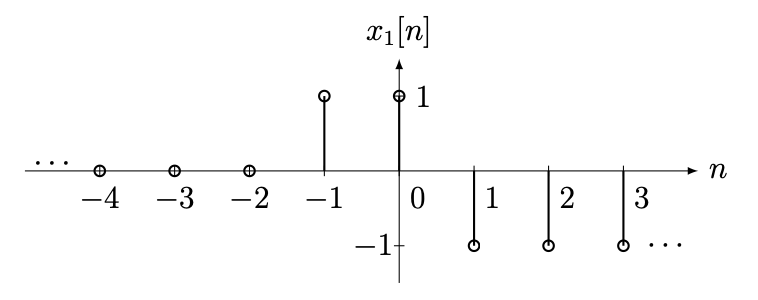
\includegraphics[width=0.7\linewidth]{docimgs/Fruehjahr_17.png}
        \end{center}
        \item[] Leiten Sie das Resultat als Funktion der Sprungantwort $a_1$ her. Begründen Sie die Schritte in Ihrer Herleitung über die Eigenschaften von LTI-Systemen.
    \end{itemize}
\end{itemize}

\vfill \null
\pagebreak

\begin{itemize}
    \item[] \begin{itemize}
        \item[iii.] Geben Sie eine allgemeine hinreichende Begründung für BIBO-Stabilität eines zeitdiskreten LTI-Systems an. Zeigen Sie mithilfe dieser Bedingung, dass $H_1$ BIBO-stabil ist.
    \end{itemize}
\end{itemize}


\begin{tikzpicture}
    % Define the box size and grid spacing
    \draw[step=0.5cm,gray!50,very thin] (0,0) grid (16.5,18
    ); % (0,0) is bottom-left corner, (10,10) is top-right corner
\end{tikzpicture}

\pagebreak

\subsection*{Differenzengleichungen}
\vspace*{-0.5cm}
Die Eingangs-Ausgangsbeziehung vieler zeitdiskreter LTI-Systeme kann mithilfe von Differenzengleichungen beschrieben werden. Diese Differenzengleichungen haben die Form:
$$\sum_{k=0}^N a_k y[n-k] = \sum_{m=0}^M b_m x[n-m]$$
Um Differenzengleichungen zu beschreiben sind Blockschaltbilder sehr hilfreich. In Blockschaltbildern verwenden wir die folgenden Elemente:\\
\vspace*{-1cm}
\begin{center}
    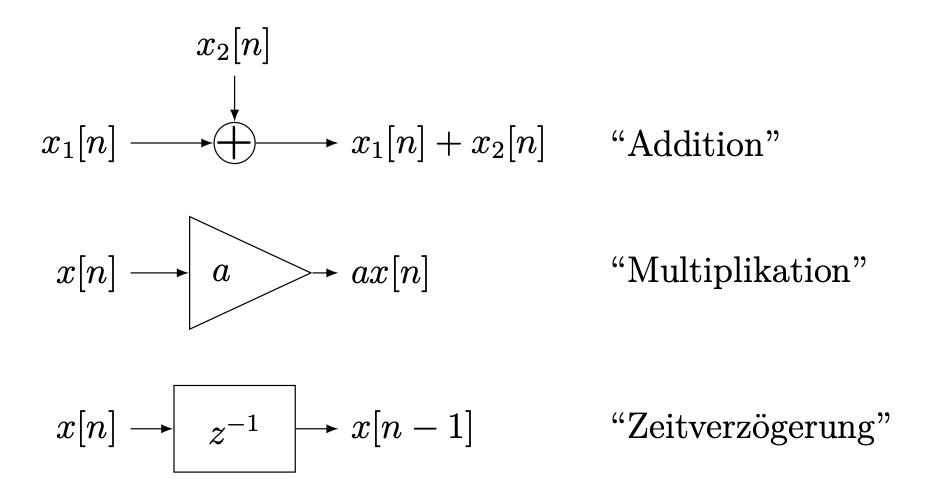
\includegraphics[width = 0.52\linewidth]{docimgs/Blockschaltbilder.png}
\end{center}
\vspace*{-0.5cm}
Wenn wir obige Differenzengleichung umformen, erhalten wir:
$$a_0 y[n] + \sum_{k=1}^N a_k y[n-k] = \sum_{m=0}^M b_m x[n-m] \implies y[n] = -\sum_{k=1}^N \frac{a_k}{a_0}y[n-k] + \sum_{m=0}^M \frac{b_m}{a_0} x[n-m]$$
$$\text{Wir setzen } -\frac{a_k}{a_0} = \Tilde{a}_k \text{ und } \frac{b_m}{a_0} = \Tilde{b}_m \implies y[n] = \sum_{k=1}^N \Tilde{a}_k \underset{\verticaltransform{}{0.5}{}{\hat{y}(\theta)e^{-2 \pi i k \theta}}}{y[n-k]} + \sum_{m=0}^M \Tilde{b}_m \underset{\verticaltransform{}{0.5}{}{\hat{x}(\theta)e^{-2 \pi i m \theta}}}{x[n-m]} $$
\vspace*{-1cm}
\begin{center}
    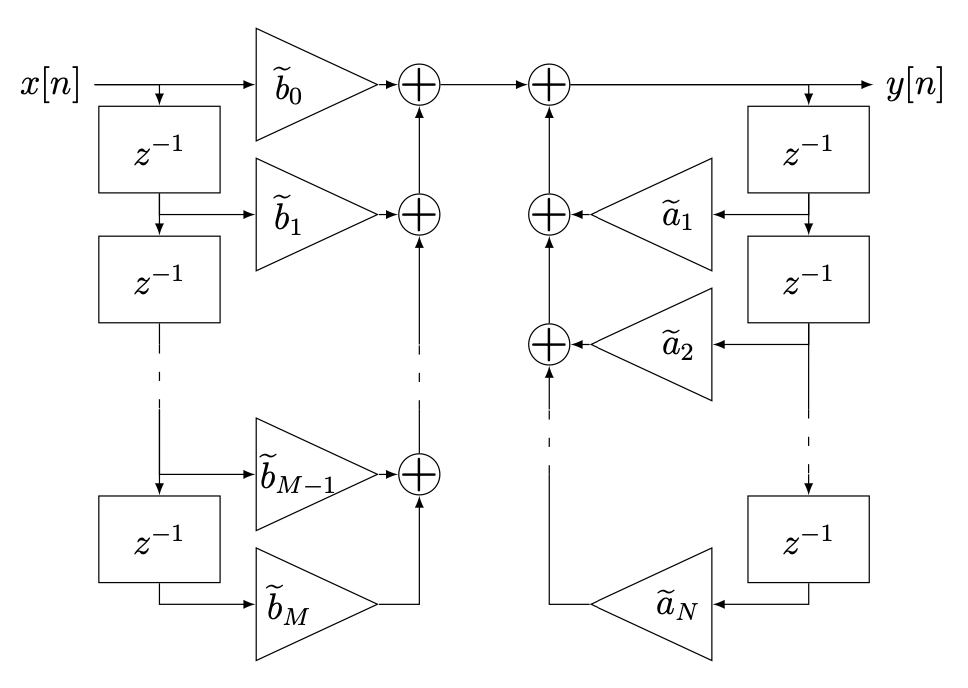
\includegraphics[width=0.6\linewidth]{docimgs/Blockschaltbild2.png}
\end{center}

\pagebreak

\subsection*{Beispiel}
\vspace*{-0.5cm}
Wir betrachten ein LTI-System beschrieben durch die Differenzengleichung:
$$2 y[n] - 3y[n-3] = x[n] + 6x[n-1] - 8x[n-7]$$
\textbf{Ziel}: Suche $\hat{h}(\theta) = \displaystyle\frac{\hat{y}(\theta)}{\hat{x}(\theta)}$. Um die Fouriertransformierte der Impulsantwort zu finden, nehmen wir die DTFT auf beiden Seiten der Differenzengleichung.
\vspace*{-0.5cm}
\begin{itemize}[leftmargin = 0pt]
    \item[] Dank $x[n-N_0] \hspace{10pt} \displaystyle\transform{55.}{1} \hspace{10pt}\displaystyle e^{-2 \pi i N_0 \theta} \hat{x}(\theta)$ haben wir: $\displaystyle\left( \displaystyle\sum_{k=0}^N a_k e^{-2\pi i k \theta}\right)\hat{y}(\theta) = \displaystyle\left( \displaystyle\sum_{m=0}^M b_m e^{-2 \pi i m \theta}\right)\hat{x}(\theta)$
    \item[] Somit $\hat{h}(\theta)= \displaystyle\frac{\hat{y}(\theta)}{\hat{x}(\theta)} = \displaystyle\frac{\displaystyle\sum_{m=0}^M b_m e^{-2 \pi i m \theta}}{ \displaystyle\sum_{k=0}^N a_k e^{-2\pi i k \theta}}
    $
\end{itemize}

\noindent
\begin{minipage}[t]{0.48\textwidth} % Left column
    \textbf{FIR-Filter (Finite Impulse Response)}\\[0.5em]
    Die Impulsantwort von FIR-Filtern hat eine \textbf{endliche Länge}. Eine Konsequenz davon ist, dass FIR-Filter keine Rückkopplungen haben.\\
    \vspace*{-0.5cm}
    \begin{center}
        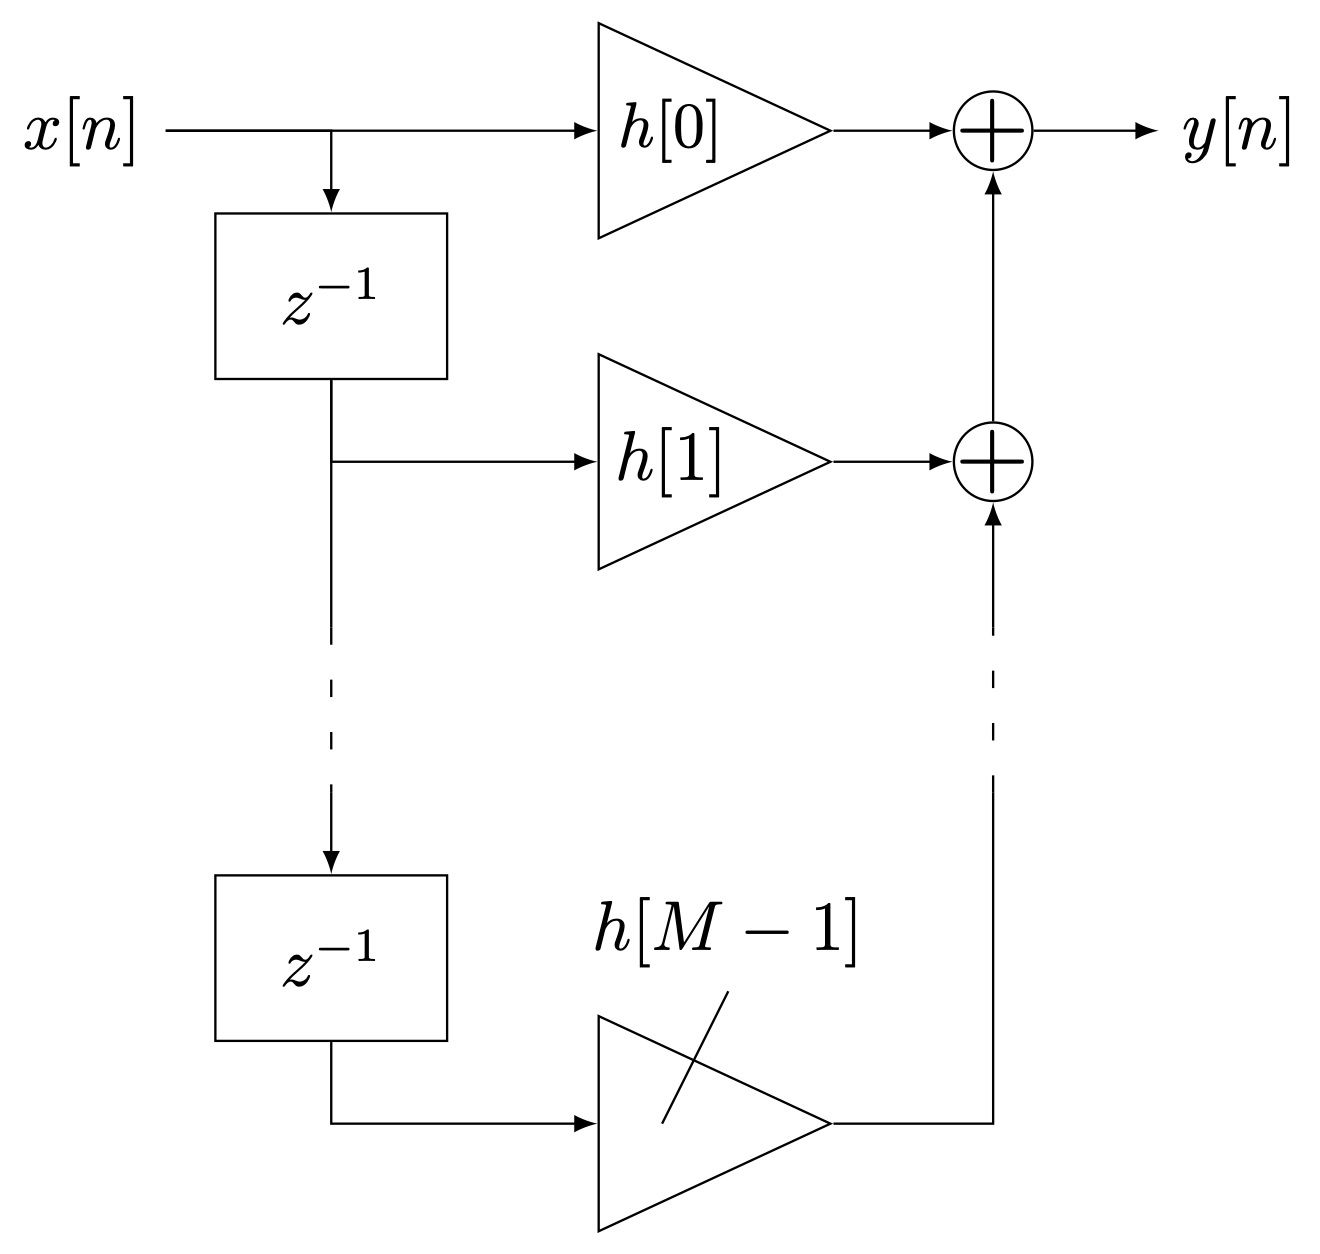
\includegraphics[width=0.7\linewidth]{docimgs/FIR.png}
    \end{center}
    $$y[n] \overset{\text{LTI}}{=} \sum_{l=-\infty}^\infty h[l] x[n-l] = \sum_{l=0}^{M-1} h[l]x[n-l] $$
    \vspace*{-0.5cm}
    \begin{center}
        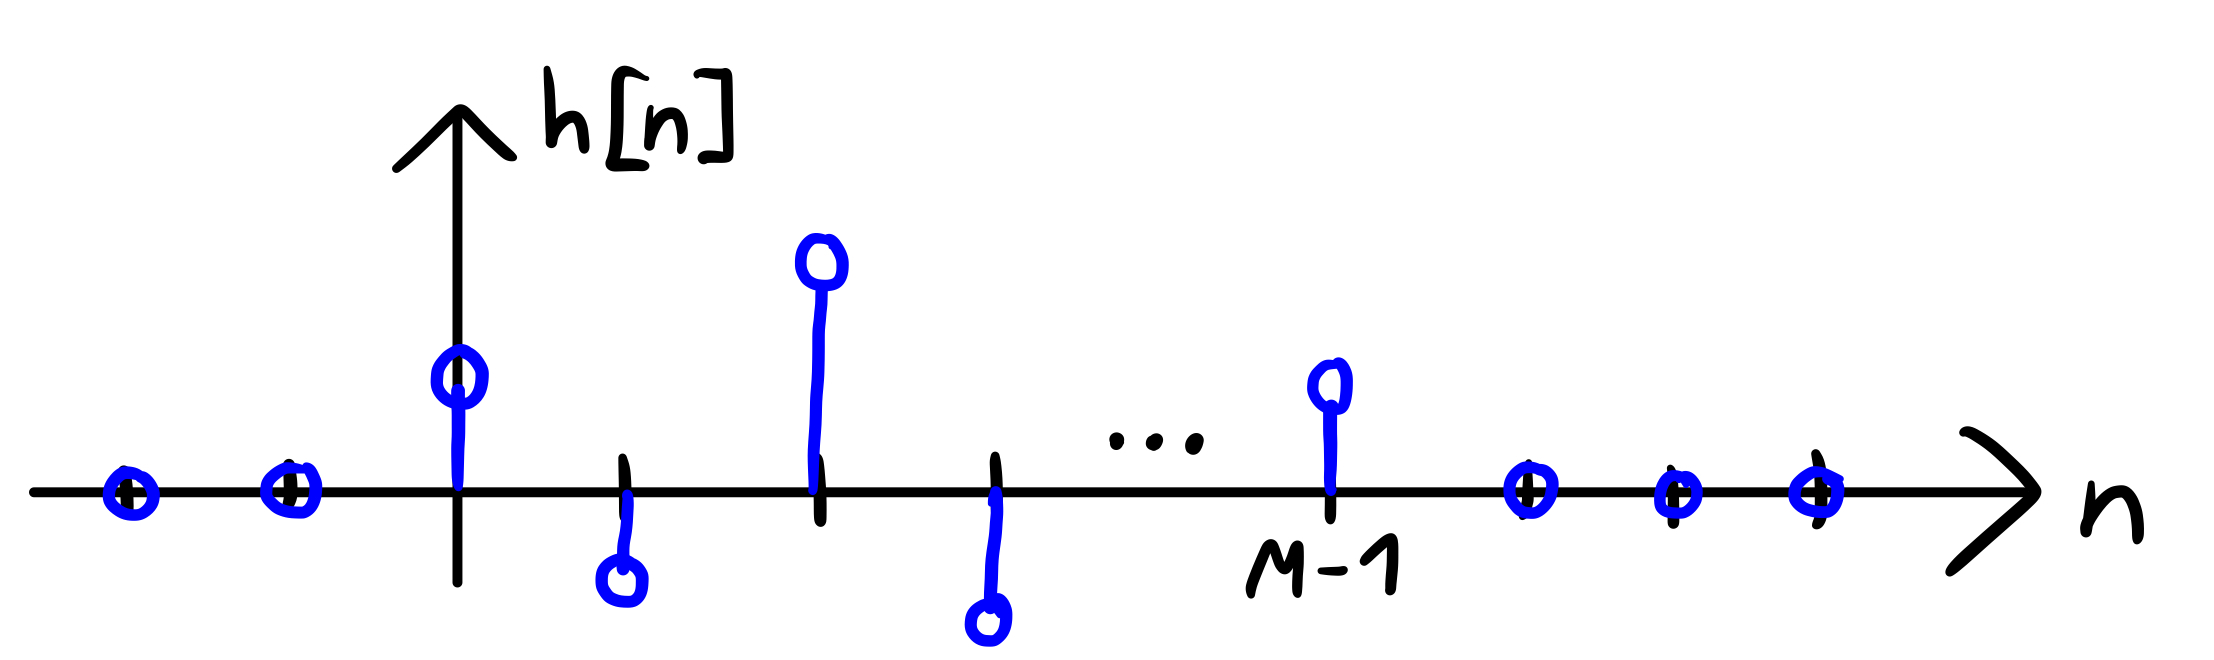
\includegraphics[width=0.8\linewidth]{docimgs/bsp_fir.jpeg}
    \end{center}
\end{minipage}
\hfill
\begin{minipage}[t]{0.48\textwidth} % Right column
    \textbf{IIR-Filter (Infinite Impulse Resplonse)}\\[0.5em]
    Die Impulsantwort von IIR-Filtern hat \textbf{unendliche Länge}. Das Blockschaltbild hat Rückkopplungen, welche oft zu Stabilitätsproblemen führen. Wenn $h[n]$ unendlich lang ist, kann es gut sein, dass die Impulsantwort nicht absolut summierbar ist.\\
    \vspace*{-0.5cm}
    \begin{center}
        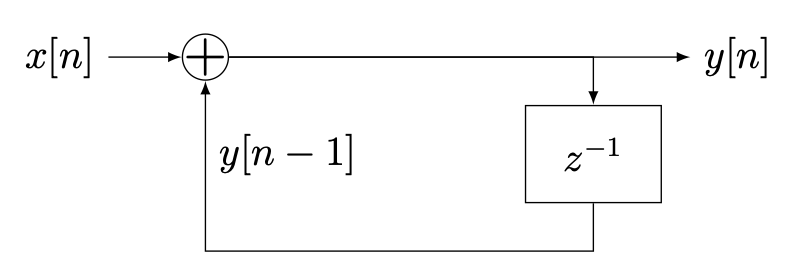
\includegraphics[width=\linewidth]{docimgs/IIR.png}
    \end{center}
    \begin{align*}
        y[n] &= x[n] + y[n-1] = x[n] + \sum_{k=-\infty}^{n-1}x[k] \\
        &= \sum_{k=-\infty}^n x[k] \overset{\text{LTI}}{=} \sum_{k=-\infty}^\infty x[k]h[n-k]
    \end{align*}
    $$\implies h[n-k] = \sigma[n-k] \Leftrightarrow h[n] = \sigma[n]$$
    Dieses System ist nicht BIBO-stabil!
\end{minipage}

\vfill \null
\pagebreak

\subsection*{Prüfungsaufgabe: Frühjahr: 2017, Aufgabe 3.b)}
\begin{itemize}
    \item[b)] (11 Punkte) Wir betrachten nun das zeitdiskrete LTI-System $H_2$ mit Frequenzgang
    $$\hat{h}_2(\theta) = \frac{7 e^{4 \pi i \theta}}{1- \frac{1}{12}e^{-2\pi i \theta} - \frac{1}{12} e^{-4 \pi i \theta}}$$
    \begin{itemize}
        \item[i.] Bestimmen Sie die Impulsantwort $h_2[n]$ von $H_2$. Ist $H_2$ kausal? Begründen Sie Ihre Antwort.
        \item[ii.] Bestimmen Sie die zu $H_2$ gehörige Differenzengleichung.
    \end{itemize}
\end{itemize}


\begin{tikzpicture}
    % Define the box size and grid spacing
    \draw[step=0.5cm,gray!50,very thin] (0,0) grid (16.5,15
    ); % (0,0) is bottom-left corner, (10,10) is top-right corner
\end{tikzpicture}

\pagebreak


\begin{tikzpicture}
    % Define the box size and grid spacing
    \draw[step=0.5cm,gray!50,very thin] (0,0) grid (16.5,21
    ); % (0,0) is bottom-left corner, (10,10) is top-right corner
\end{tikzpicture}

\end{document}